\documentclass[11pt,a4paper]{report}

\usepackage{polski}
\usepackage[utf8]{inputenc} 
\usepackage{a4wide}
\usepackage{tabularx}
\usepackage{lastpage}
\usepackage{fancyhdr}
\usepackage{graphicx}
\usepackage{caption}
\usepackage{latexsym}

% strona tytułowa
\begin{titlepage}
\title{\Huge Specyfikacja Implementacyjna  Projektu\\\textsl{,,Tanks''}}
\author{Daniel Ślusarczyk i Jakub Łaba}
\date{28.04.2021}
\end {titlepage}

\renewcommand{\footrulewidth}{0pt}
\begin{document}
\maketitle

% zmiana numeracji sekcji 0.X -> X
\renewcommand*\thesection{\arabic{section}} 


% numeracja stron
\pagestyle{fancy}
\fancyhf{}
\rhead{\textsl{Specyfikacja Implementacyjna ,,Tanks" | D. Ślusarczyk, J. Łaba}}
\rfoot{Strona \thepage \hspace{1pt} z \pageref{LastPage}}
\setcounter{page}{0}

% spis treści bez numeracji stron
\fancypagestyle{plain}
{
\fancyhead{} 
\fancyfoot{} 
}
\thispagestyle{empty} 
\tableofcontents 
\thispagestyle{empty}
\newpage

\fancypagestyle{plain} 
{
\fancyhead{} 
\fancyfoot[C]{\thepage}
}


% pierwsza sekcja
\section{Informacje ogólne}\label{sec:tekst}
\subsection {Przeznaczenie dokumentu}
Specyfikacja implementacyjna projektu „Tanks” jest dokumentem omawiającym tematykę przedstawianego oprogramowania pod kątem implementacji. Wyjaśnia takie aspekty programu jak jego budowę, przeprowadzanie testów i podejście konceptualne przyświecające procesowi tworzenia. Dokument ten stanowi źródło wiedzy dla osób zainteresowanych działaniem oprogramowania \textsl{Tanks}.
\subsection {Zarys problematyki}
„Tanks” to gra oparta na rywalizacji dwóch graczy mających do dyspozycji po jednym czołgu rozmieszczonym na lewym lub prawym brzegu pola bitwy, których ruch ogranicza się do poruszania w górę i w dół, oraz obracania lufą +/- 60 stopni. W czasie trwania rozgrywki przez środkową część pola przemieszczają się komórki z określoną prędkością należące do jednej z grup:
\begin{itemize}
\item {Zwykła komórka} -- kwadrat o określonym boku o wszystkich krawędziach wrażliwych na kontakt. Każde unicestwienie komórki to punkty dla gracza, który tego dokonał
\item {Komórka bomba} -- kwadrat o określonym boku o górnej krawędzi wrażliwej na kontakt. Unicestwienie komórki pozwala przerwać grę.
\item {Kolonia} -- zbiór maksymalnie 5 komórek w określonym ustawieniu. Unicestwienie ostatniej komórki w kolonii powoduje przyznanie punktów za wszystkie komórki graczowi, który tego dokonał.
\end{itemize}
Każda komórka ma określony poziom kontaktów z pociskami potrzebnych do jej unicestwienia.
Komórka może zostać trafiona za pomocą okrągłego pocisku o ustalonym promieniu, wystrzeliwanym z pojazdu każdego gracza. Na polu bitwy można znajdować się ograniczona ilość pocisków jednego z graczy. Dodatkowo co określony przedział czasu zwiększane są: szybkość pocisków i przemieszczania się komórek, oraz ilość kontaktów z pociskiem potrzebnych do unicestwienia komórki. W tym samym czasie zmniejszany jest promień wystrzeliwanych pocisków i długość boków komórek.
Koniec rozgrywki może zostać osiągnięty po przekroczeniu ustalonego czasu gry, lub zniszczeniu komórki bomby – wygrywa gracz z większą ilością punktów.


\subsection {Środowisko powstawania}
Program \textsl{,,Tanks''} jest napisany w obiektowym języku programowania Java. Zintegrowanym środowiskiem programistycznym używanym w procesie tworzenia aplikacji jest „IntelliJ IDEA” (IDE dla Javy firmy JetBrains). Dokładnie wersje środowiska programistycznego:\\
\begin{tabularx}{\textwidth}{  X|Xl  }
 \hline
 \\Element środowiska                                   					& Wersja\\
 \hline \hline
			\\Język programowania			&Java SE 16\\
 \hline
			\\Java Development Kit			&10.0.1 / 17\\
 \hline
			\\IntelliJ IDEA				&2020.3.3 dla Windowsa\\
\hline 
			\\Apache Maven 				&3.8.1\\
 \hline
\end{tabularx}
\subsubsection {Framework graficzny}
Proces tworzenia oprogramowania jest oparty o framework graficzny \textsl{JavaFX} w wersji 11.0.2.

% druga sekcja
\section{Budowa programu}\label{sec:tekst}

\subsection {Wzorzec projektowy}
Projekt \textsl{,,Tanks''} jest oparty na strukturalnym wzorcu projektowym – \textsl{Fasada}. Jego realizacja przebiega poprzez możliwie maksymalne oddzielenie użytkownika od złożoności całego systemu i eksponowanie poprzez interfejs graficzny możliwości, których klient naprawdę potrzebuje. Rolę klasy utożsamianą z fasadą pełni w projekcie klasa \textsl{GameClient} udzielająca ograniczony dostęp do złożonych metod podsystemu. 

\subsection {Zaimplementowane klasy}
\subsubsection{GameClient}
Jedyna klasa, z którą w bezpośrednią interakcję wchodzi użytkownik. Odpowiada za interfejs graficzny aplikacji oraz sterowanie przekazywaniem informacji o wciśniętych klawiszach do kolejnych klas, w celu zrealizowania sterowania czołgami.

\subsubsection{Bomb}
Klasa, która sama w sobie przechowuje informacje o komórce-- bombie oraz w odpowiedni sposób realizuje kolizję pocisków z jej jedyną wrażliwą ścianą. Istnieje tylko jedna bomba, więc instancje tej klasy nie są tworzone - wszystkie pola są statyczne, a kontruktor prywatny.

\subsubsection{GameBoard}
W tej klasie odbywa się główne sterowanie komponentami gry – ruchami oraz zmianami rozmiarów komórek i pocisków, generowaniem kolonii, rozpatrywaniem trafień w komórki i adekwatnym przyznawaniem punktów odpowiedniemu graczowi. 

\subsubsection{PlayerInfo}
Pozwala na zarządzanie pojedynczym graczem poprzez przypisanie mu czołgu oraz przyznawanie mu punktów.

\subsubsection{Tank}
Pozwala na zarządzanie pojedynczym czołgiem poprzez przechowywanie informacji o wystrzelonych pociskach oraz metody umożliwiające ruch czołgu, przechył lufy oraz oddawanie strzałów.

\subsubsection{GameSegment}
Klasa abstrakcyjna wprowadzona w celu generalizacji pewnych cech wspólnych klas \textsl{Cell} oraz \textsl{Bullet}.

\subsubsection{Cell}
Reprezentacja pojedynczej komórki, będąca rozszerzeniem abstrakcji GameSegment, zawierająca jej typ, ilość punktów życia oraz posiadająca metodę umożliwiającą uszkodzenie jej.

\subsubsection{Bullet}
Reprezentacja pojedynczego pocisku, będąca rozszerzeniem abstrakcji GameSegment. Zawiera jedynie informacje o niemodyfikowalnym wektorze opisującym tor ruchu danego pocisku.

\subsubsection{Colony}
Umożliwia łączenie komórek w kolonie i rozpatrywanie owego zbioru jako spójnej całości.
\newpage
\subsection{Diagram klas}
 \begin{figure}[!ht]
\centerline{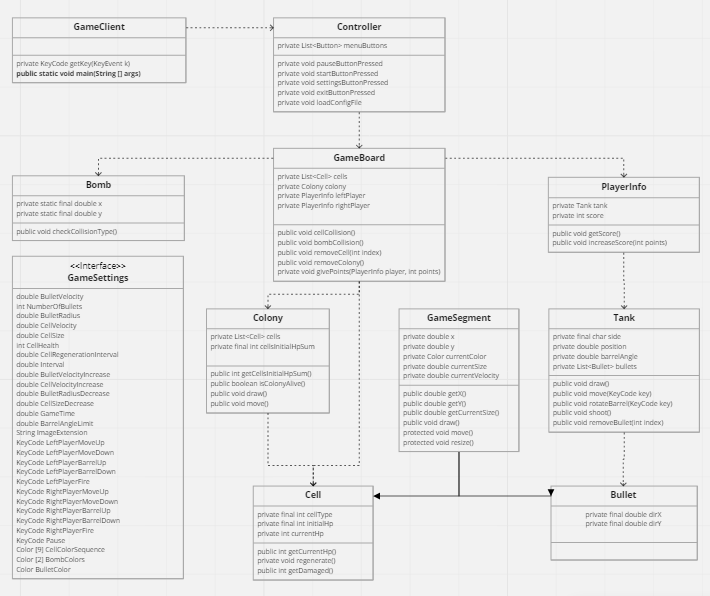
\includegraphics{img/classDiagram.png}}
\caption{Diagram klas UML}
\end{figure}
\newpage
% trzecia sekcja
\section{Testowanie}
Testowanie aplikacji \textsl{,,Tanks''} będzie przeprowadzane za pomocą automatycznych testów jednostkowych z wykorzystaniem frameworku JUnit.
Zakres testów będzie obejmował najważniejsze funkcjonalności kluczowych komponentów gry oraz kluczowych interakcji pomiędzy nimi. Testowana będzie również poprawność wykrywania odpowiednich błędów podczas wczytywania nieodpowiednio sformatowanego pliku konfiguracyjnego.

% czwarta sekcja
\section{Kod programu}
\subsection {Koncepcje nazewnicze}
Pisanie kodu zespołowo w języku obiektowym Java wymaga przyjęcia wspólnej koncepcji nazewniczej w celu uzyskania przejrzystego i czytelnego kodu. Cały kod w obrębie projektu powinien być napisany w sposób zapewniający zachowanie następujących zasad:\\
\begin{itemize}
\item{}Wszystkie nazwy są w języku angielskim,
\item{}Nazwy zmiennych i metod zaczynają się z małych liter, a każde kolejne słowo, które zawierają rozpoczyna się z wielkiej litery np. leftPlayer, initialHp. Nazwy klas powinny być jasno utożsamiane z obiektem, którego dotyczą, z zachowaniem adekwatnego poziomu abstrakcji.
\item{}Każde zagłębienie w kodzie jest symbolizowane przez rosnący akapit
\item{}Znaki rozpoczynające dany blok instrukcji znajdują się w jednej linii z nazwą metody, instrukcji warunkowej lub pętli, jeśli to możliwe
\item{}Adnotacje znajdują się w oddzielnym wierszu, bezpośrednio poprzedzającym metodę, do której się odnoszą (\textsl{@Override}, \textsl{@Test}, etc.)
\end{itemize}

\subsection {Sposób wprowadzania zmian}
Każdy członek zespołu dokonuje zmian w obrębie kodu, za który odpowiada lub kodu, za który nie odpowiada po uprzedniej konsultacji z autorem. Niemniej jednak, każda wprowadzana zmiana powinna zachowywać zasady przyjęte przy procesie tworzenia i nie zaburzać czytelności kodu.
\subsection {System kontroli wersji}
System kontroli wersji jest narzędziem używanym przez cały proces tworzenia oprogramowania. Każda znacząca zmiana dokonywana przez osobę z zespołu jest umieszczana na osobnej \textsl{gałęzi} w repozytorium, a następnie podczas spotkania zespołu jest scalana z główną wersją znajdującą się na gałęzi \textsl{master}. Proces ten przebiega przy użyciu systemu kontroli wersji “GitHub”.
\subsection {Struktura plików}
Cały projekt mieście się w obrębie folderu \textsl{ProjectTanks}, który dzieli się na trzy podfoldery: \textsl{Screenshots} (przechowuje zdjęcia powstałe w wyniku funkcjonalności programu jaką jest tworzenie grafiki po zakończonej rozgrywce, \textsl{ConfigFiles} (przechowuje pliki konfiguracyjne), oraz \textsl{source}. Ostatni z nich zawiera pliki z rozszerzeniem \textsl{.java} lub \textsl{.fxml}, oraz folder \textsl{graphicsElem} zawierający grafiki potrzebne do tworzenia programu.
 \begin{figure}[!ht]
\centerline{\includegraphics{img/FileStructure.png}}
\caption{Struktura plików projektu}
\end{figure}



\end{document}